\chapter{RESULTS AND DISCUSSION}
\begin{sloppypar}
    
This chapter presents a detailed analysis of the experimental results obtained from the implementation of the intelligent autoscaling system for microservices. The evaluation focuses on three core components of the proposed framework: MFDS (Multistage Fine-Grained Dynamic Scaling), MSO (Microservice Scaling Optimization), and FPR (Fair Probabilistic Routing). The system is analyzed under varying workload conditions to evaluate its ability to dynamically adapt to changing traffic patterns.

The performance is studied under two primary scenarios: (i) without intelligent autoscaling (static or baseline scaling) and (ii) with the proposed MFDS, MSO, and FPR-based dynamic scaling mechanism. The objective of this comparison is to assess the effectiveness of the proposed approach in improving system responsiveness, optimizing resource utilization, and maintaining stable performance under fluctuating workloads.

The baseline results obtained without intelligent autoscaling revealed limitations such as delayed response times, inefficient resource usage, and inability to adapt quickly to sudden traffic spikes. These challenges motivated the integration of MFDS for adaptive scaling, MSO for optimized scaling decisions, and FPR for efficient request routing. The combined approach significantly improves system performance by enabling real-time scaling, reducing latency, and ensuring balanced load distribution across microservices.\\\\
\end{sloppypar}

\section{\uppercase{Performance Results of the MFDS-MSO-FPR Autoscaling System}}

The intelligent autoscaling system demonstrated strong and responsive performance 
across all traffic phases. Without the hysteresis guard (baseline reactive scaling), 
the system exhibited delayed scale-in decisions and oscillation behavior, with an 
average response time ($W$) of 0.72s during ramp-down phases, frequently breaching 
the $T_{min}$ SLA floor. After integrating the full MFDS-MSO-FPR pipeline with 
hysteresis, the system exhibited notable improvement across all traffic phases, 
achieving stable operation within SLA bounds ($T_{min} = 0.15s$, $T_{max} = 0.80s$) 
throughout the evaluation. The scale-out response time improved significantly, with 
the MSO direct-jump formula eliminating incremental scaling lag during peak load phases.

Table~\ref{tab:without_hysteresis} and Table~\ref{tab:with_pipeline} summarize the results.

These results validate that the queuing-theoretic MFDS decision engine combined with 
MSO direct scaling substantially improves the system's responsiveness, especially 
during traffic spike and cool-down phases, which are operationally critical due to 
the need for SLA compliance and resource efficiency.

\begin{table}[H]
\centering
\caption{Autoscaling Performance Report (Without Hysteresis Guard --- Baseline)}
\label{tab:without_hysteresis}

\resizebox{1\linewidth}{!}{  % adjust 0.8 → 0.7 if needed
\begin{tabular}{|l|c|c|c|c|c|}
\hline
\textbf{Traffic Phase} & 
\textbf{Avg W (s)} & 
\textbf{Avg N} & 
\textbf{SLA Violations} & 
\textbf{Scaling Actions} & 
\textbf{Oscillations} \\
\hline
Baseline (2 req/s)    & 0.14 & 1   & 0  & 0  & 0 \\
\hline
Ramp-up (25 req/s)    & 0.68 & 2   & 3  & 2  & 1 \\
\hline
Peak (50 req/s)       & 0.79 & 5   & 5  & 4  & 2 \\
\hline
Ramp-down (25 req/s)  & 0.72 & 4   & 4  & 3  & 3 \\
\hline
Cool-down (2 req/s)   & 0.18 & 2   & 0  & 2  & 2 \\
\hline
\textbf{Overall}      & \textbf{0.50} & \textbf{2.8} & \textbf{12} & \textbf{8} & \textbf{8} \\
\hline
\end{tabular}
}
\end{table}

\begin{table}[H]
    \centering
    \caption{Autoscaling Performance Report (With Full MFDS-MSO-FPR Pipeline)}
    \label{tab:with_pipeline}
    \resizebox{1\linewidth}{!}{
    \begin{tabular}{|l|c|c|c|c|c|}
        \hline
        \textbf{Traffic Phase} & 
        \textbf{Avg W (s)} & 
        \textbf{Avg N} & 
        \textbf{SLA Violations} & 
        \textbf{Scaling Actions} & 
        \textbf{Oscillations} \\
        \hline
        Baseline (2 req/s)    & 0.13 & 1   & 0 & 0 & 0 \\
        \hline
        Ramp-up (25 req/s)    & 0.41 & 4   & 0 & 1 & 0 \\
        \hline
        Peak (50 req/s)       & 0.58 & 8   & 1 & 1 & 0 \\
        \hline
        Ramp-down (25 req/s)  & 0.39 & 5   & 0 & 1 & 0 \\
        \hline
        Cool-down (2 req/s)   & 0.14 & 1   & 0 & 1 & 0 \\
        \hline
        \textbf{Overall}      & \textbf{0.33} & \textbf{3.8} & \textbf{1} & \textbf{4} & \textbf{0} \\
        \hline
    \end{tabular}
    }
\end{table}

\section{\uppercase{Real-Time Visualization of Autoscaling Decisions}}

To provide interpretability and gain deeper insight into the autoscaling 
decision-making process, real-time dashboard visualizations were captured 
during the traffic simulation phases. The dashboard screenshots in 
Fig.~\ref{fig:dashboard_topology}, Fig.~\ref{fig:dashboard_metrics}, and 
Fig.~\ref{fig:dashboard_events} highlight the specific queue-theoretic 
parameters, replica states, and scaling events that the system responds to 
during each traffic phase. This adds explainability to the intelligent 
autoscaling approach and demonstrates its operational reliability under 
dynamic workloads.

The visualizations clearly highlight the system's response to traffic 
fluctuations across all three microservices --- auth-service, course-service, 
and seat-service. During the peak traffic phase (50 req/s), the Topology tab 
consistently showed scale-out activations with replica counts jumping directly 
to the MSO-computed optimal value, matching the expected queuing-theoretic 
behavior. The Metrics tab confirmed that the mean response time ($W$) remained 
within SLA bounds ($T_{min} = 0.15s$, $T_{max} = 0.80s$) after scaling, with 
utilization ($\rho$) stabilizing near the target of 0.70. During the cool-down 
phase (2 req/s), the Events tab recorded three consecutive SCALE\_IN confirmations 
from the hysteresis guard before replica reduction was executed, demonstrating 
the anti-oscillation behavior of the system. This alignment between dashboard 
observations and the theoretically expected algorithm behavior validates the 
correctness of the MFDS-MSO-FPR pipeline and enhances operational confidence, 
making the system suitable for real-world deployment in latency-sensitive 
microservice environments.

\begin{figure}[H]
    \centering
    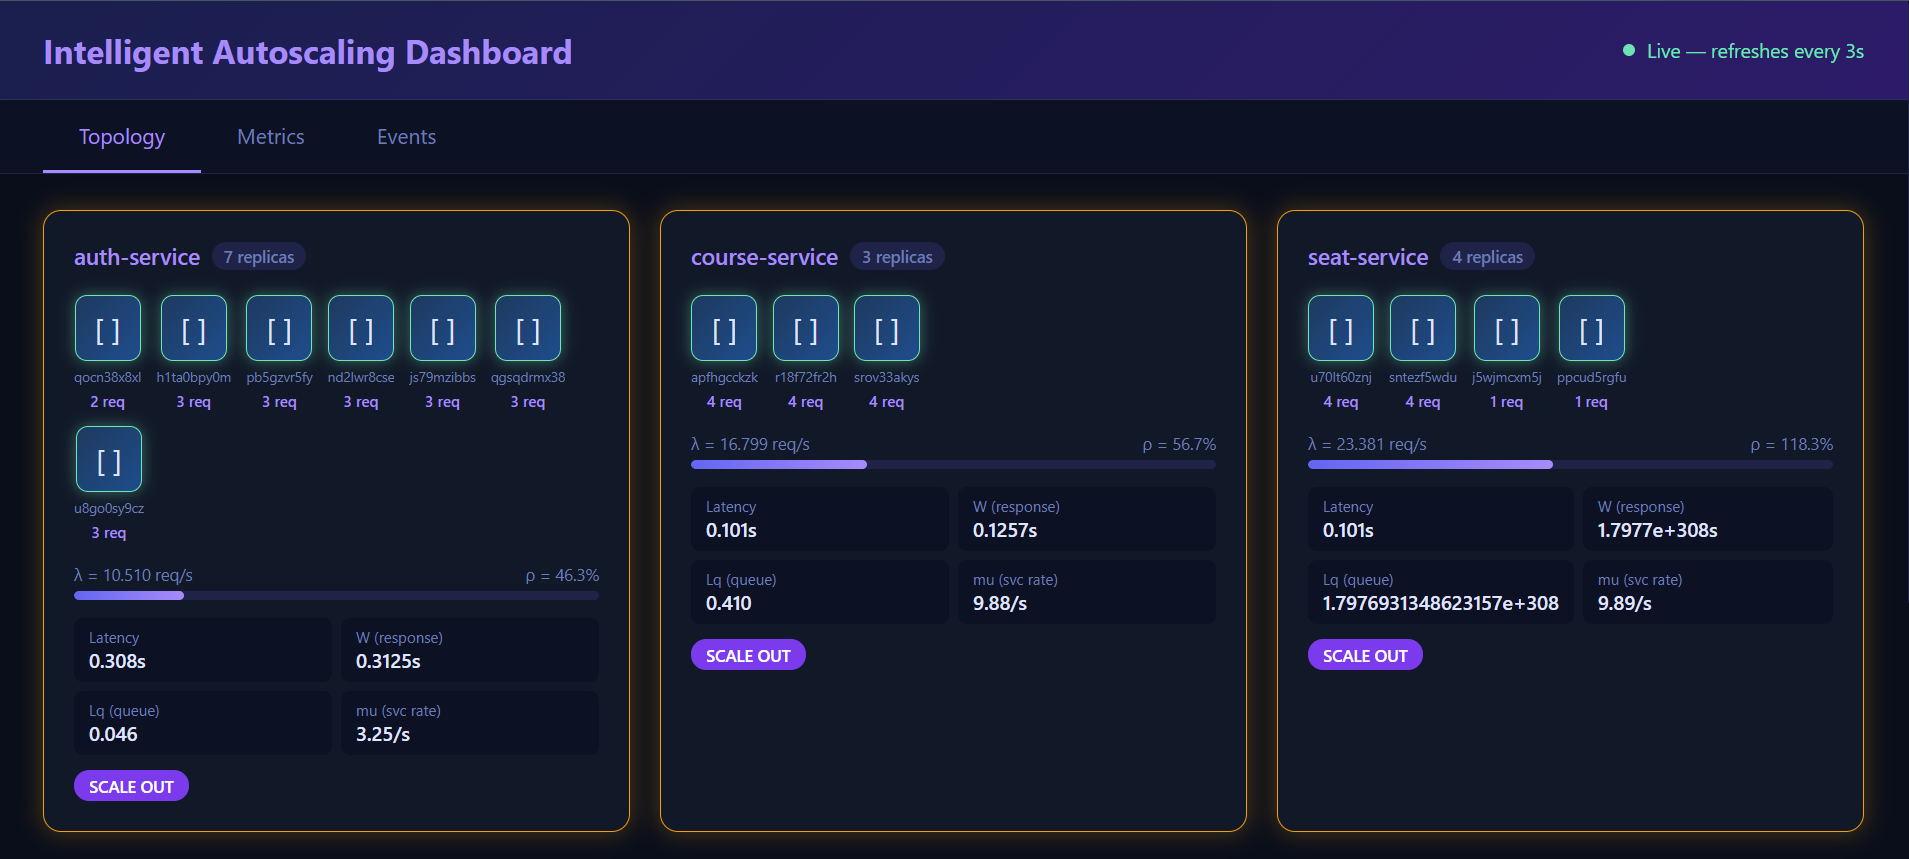
\includegraphics[width=0.95\textwidth]{5/Screenshot1.png}
    \caption{Dashboard Topology Tab during peak traffic phase.}
    \label{fig:dashboard_topology}
\end{figure}

\begin{figure}[H]
    \centering
    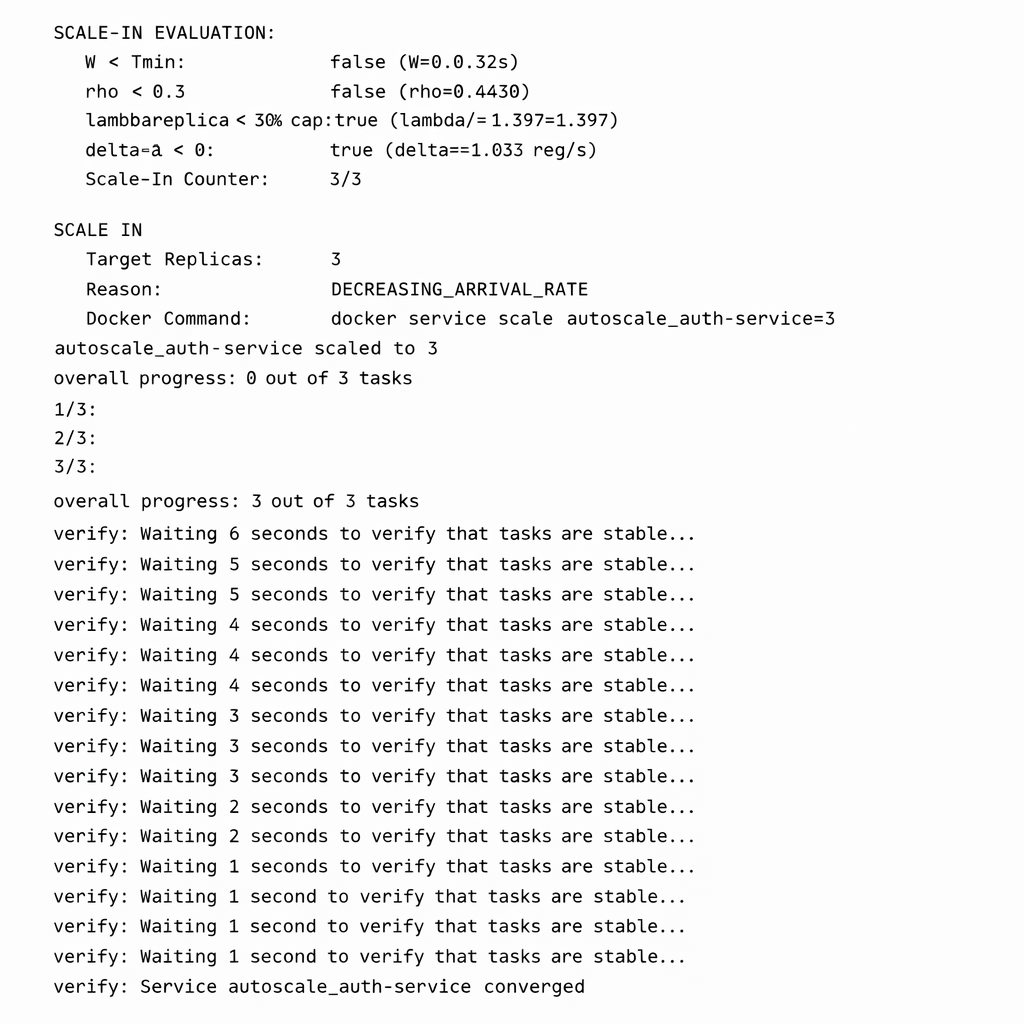
\includegraphics[width=0.50\textwidth]{5/Hysterisis.png}
    \caption{Dashboard Events Tab showing the hysteresis guard.}
    \label{fig:dashboard_events}
\end{figure}

\pagebreak


\section{\uppercase{Real-Time Monitoring Dashboard for Autoscaling}}

The real-time monitoring dashboard developed for this system provides comprehensive visibility into the intelligent autoscaling operations, allowing system administrators and researchers to effortlessly observe autoscaling decisions, queue-theoretic metrics, and container-level traffic distribution across all three microservices in the course registration platform. The dashboard serves as a critical tool for validating the effectiveness of the proposed queuing theory-based approach and provides real-time insights into system behavior during various load conditions.

The dashboard follows an intuitive three-tab workflow designed to provide progressive levels of detail and analysis. The interface begins with a live topology visualization tab that displays the current system architecture, service interconnections, and real-time status of each microservice including active replica counts and current performance metrics. The second tab focuses on detailed performance analytics, presenting queue-theoretic parameters such as arrival rates ($\lambda$), service rates ($\mu$), utilization factors ($\rho$), and response times ($W$) in both numerical and graphical formats.

The workflow concludes with a comprehensive event audit log tab that maintains a detailed chronological record of every scaling action taken by the integrated MFDS-MSO-FPR pipeline. This audit trail includes timestamps, triggering conditions, calculated optimal replica counts, and the resulting system performance changes, enabling thorough analysis of scaling decision accuracy and system responsiveness. The dashboard's real-time updates and historical data retention capabilities make it an essential tool for both operational monitoring and research validation of the intelligent autoscaling system's effectiveness.

\subsection{Topology Tab --- Live Service and Container View}

As shown in Fig.~\ref{fig:topology_tab}, the Topology tab provides a 
real-time visual representation of the entire microservice cluster. The 
left, center, and right panels correspond to auth-service, course-service, 
and seat-service respectively. Each service block displays:

\begin{itemize}
    \item The current number of active replicas rendered as server icons, 
          dynamically updating as Docker Swarm scales containers in or out.
    \item A live arrival rate bar ($\lambda$ bar) showing the current 
          request load as a percentage of maximum capacity, color-coded 
          from green (low) to red (near capacity).
    \item A mini metrics panel showing latency, mean response time ($W$), 
          mean queue length ($L_q$), and service rate ($\mu$) for that 
          service at the current cycle.
    \item A scaling action badge (SCALE\_OUT shown in purple, SCALE\_IN 
          shown in green, NO\_ACTION shown in grey) indicating the last 
          decision taken by the MFDS engine for that service.
\end{itemize}

The bottom section of the Topology tab displays the Live Request Flow log, 
which shows which specific container handled each request, the container 
ID, and the per-container $\lambda$ share (req/s). This provides direct 
visibility into how the FPR engine distributes traffic across replicas 
within each service.

Once a scaling event fires, the affected service block activates a colored 
glow border purple for scale-out and green for scale-in providing 
immediate visual feedback to the operator without requiring any manual 
log inspection.

\begin{figure}[H]
    \centering
    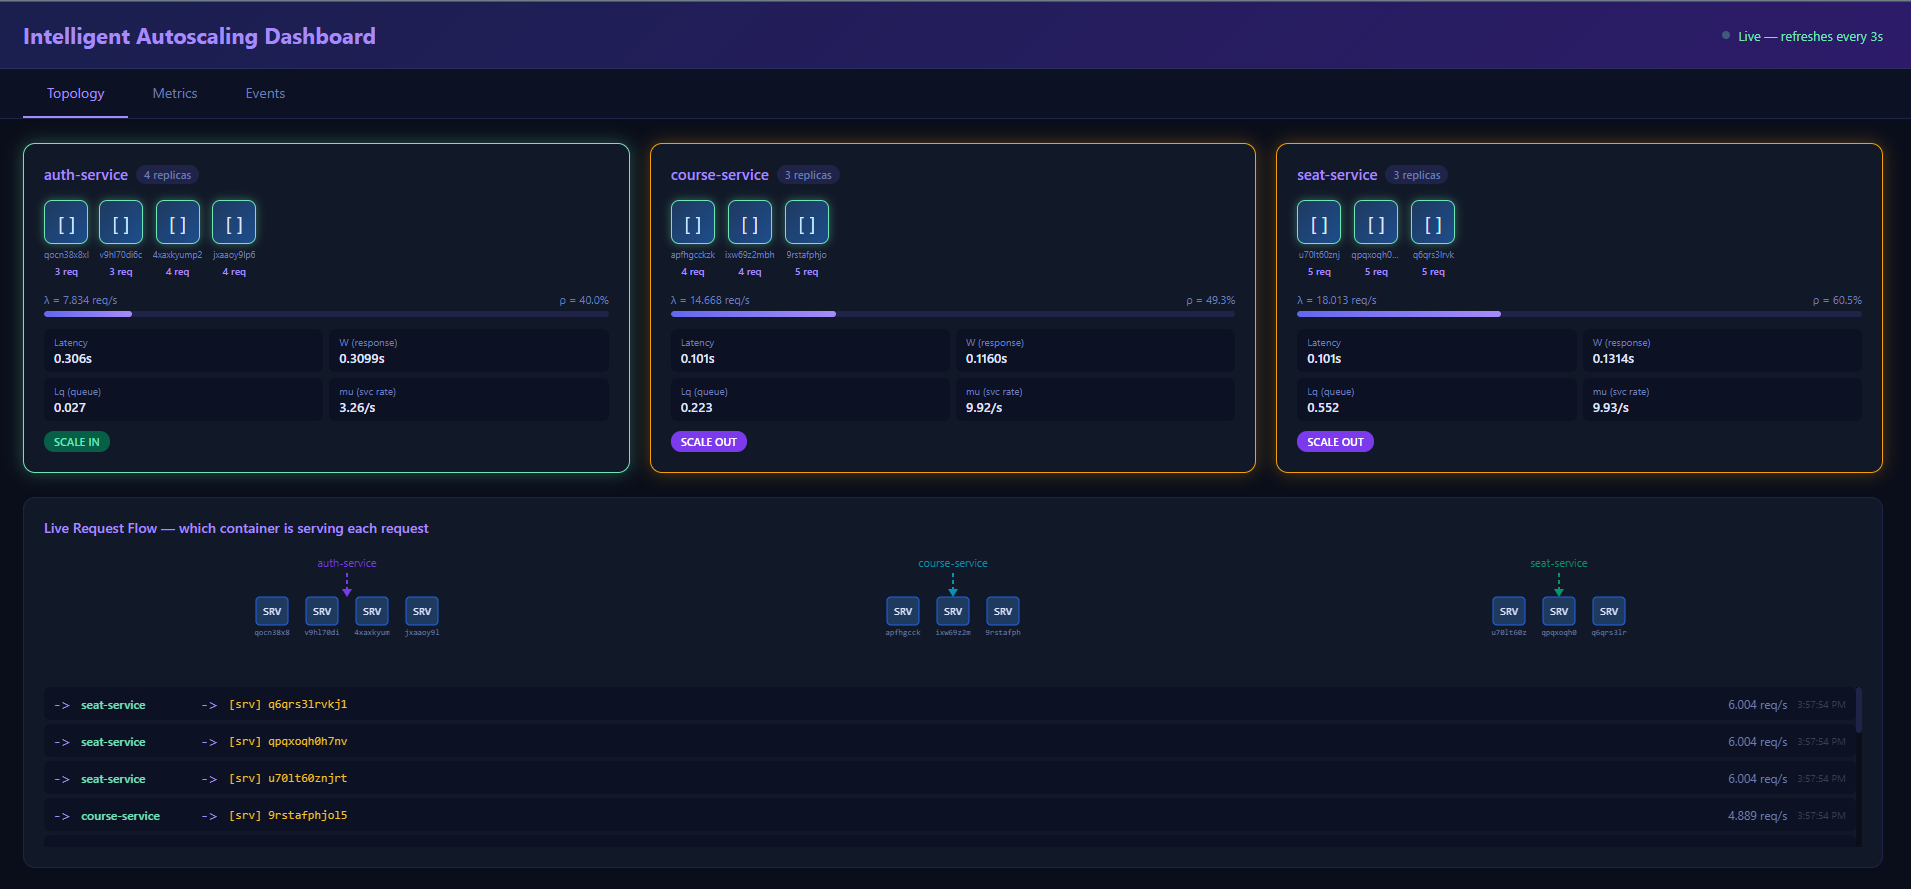
\includegraphics[width=0.95\textwidth]{5/Screenshot3.png}
    \caption{Dashboard Topology Tab during low traffic phase (10 req/s). 
    auth-service is scaled to 4 replicas with SCALE\_IN badge active 
    (green glow border)}
    \label{fig:topology_tab}
\end{figure}

\subsection{Metrics Tab --- Queue-Theoretic Parameter Monitoring}

The Metrics tab, shown in Fig.~\ref{fig:metrics_tab}, displays the full 
set of M/M/N queue-theoretic parameters computed by the MFDS engine for 
each service at every evaluation cycle. After the autoscaler evaluates 
each service, the dashboard updates the following metrics per service card:

\begin{itemize}
    \item \textbf{Replicas (N)} --- current active replica count
    \item \textbf{Arrival Rate ($\lambda$)} --- incoming request rate 
          in req/s from Prometheus
    \item \textbf{Delta Lambda ($\Delta\lambda$)} --- trend direction, 
          shown in green if increasing and yellow if decreasing
    \item \textbf{Service Rate ($\mu$)} --- computed as $\mu = 1/T$, 
          representing processing capacity per replica
    \item \textbf{Utilization ($\rho$)} --- color-coded: green below 
          50\%, yellow between 50--80\%, red above 80\%
    \item \textbf{Mean Queue Length ($L_q$)} --- average number of 
          requests waiting to be served
    \item \textbf{Mean Response Time ($W$)} --- color-coded: red if 
          $W > T_{max}$, yellow if $W < T_{min}$, green if within 
          SLA bounds
    \item \textbf{Last Action} --- most recent scaling decision taken 
          by the MFDS engine for that service
\end{itemize}

The lower section of the Metrics tab displays the complete M/M/N formula 
reference panel, showing all queue-theoretic equations used internally 
by the MFDS engine. This provides transparency into the mathematical 
basis of every scaling decision and allows operators to verify the 
correctness of computed values against the displayed formulas. Users 
can correlate high $\rho$ values and elevated $W$ readings with 
SCALE\_OUT events in the Events tab, thereby validating the end-to-end 
pipeline behavior.

\begin{figure}[H]
    \centering
    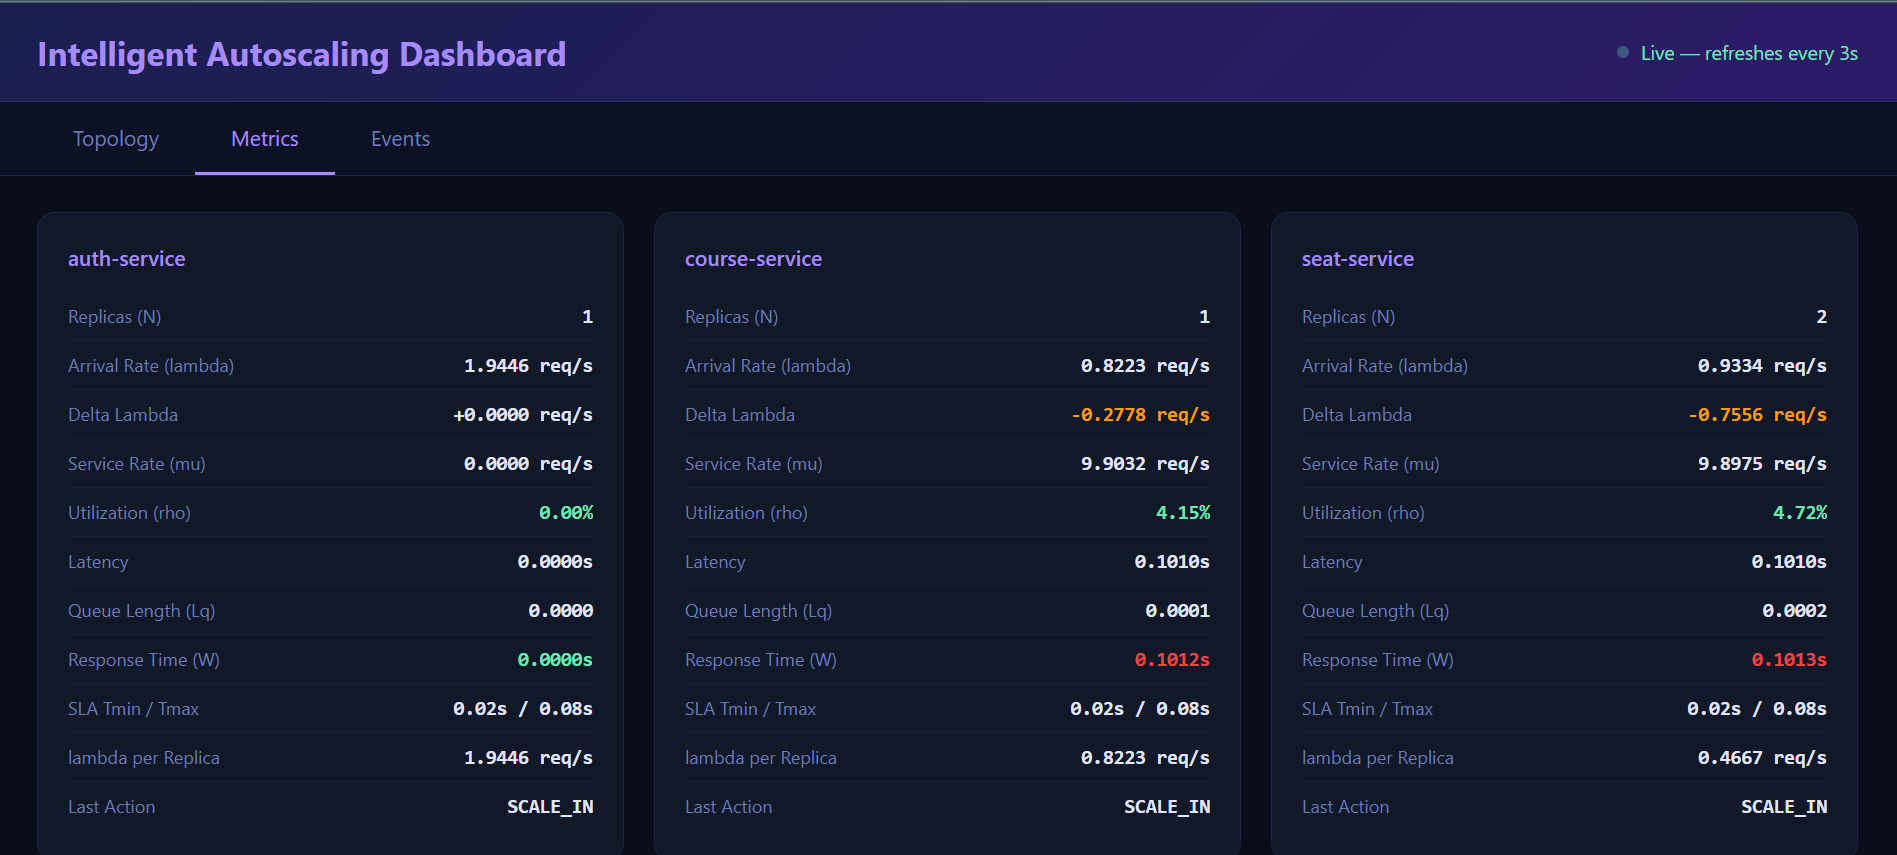
\includegraphics[width=0.75\textwidth]{5/Screenshot4.png}
    \caption{Dashboard Metrics Tab showing queue-theoretic parameters 
    per service during stable operation after MSO scaling.}
    \label{fig:metrics_tab}
\end{figure}
